\documentclass[11pt]{article}

\usepackage[margin=1in]{geometry}
\usepackage{amsmath,amssymb,amsthm}
\usepackage{booktabs}
\usepackage{graphicx}
\usepackage{xcolor}
\usepackage{algorithm}
\usepackage{algpseudocode}
\usepackage{hyperref}
\hypersetup{colorlinks=true,linkcolor=blue,citecolor=blue,urlcolor=blue}
\usepackage{newunicodechar}
\newunicodechar{α}{\ensuremath{\alpha}}  % generated tables may contain literal α

\newcommand{\R}{\mathbb{R}}
\newcommand{\code}{\mathbf{C}}
\newcommand{\softmax}{\operatorname{softmax}}
\newcommand{\maxpool}{\operatorname{maxpool}}
\newcommand{\upnn}{\operatorname{up}}
\newcommand{\NonOv}{\mathrm{NonOverlap}}

\title{\textbf{Non-Overlapping Sparsification of Motif Filters}\\[2pt]
\large A differentiable max-unpool operator at the inference-code layer}
\author{MotifInference \,---\, internal experiment report}
\date{\today}

\begin{document}
\maketitle

\begin{abstract}
We add a differentiable operator to the \texttt{MotifInference} CNN that, at a single
designated layer (the \emph{inference-code layer}), forces the receptive fields of that
layer's filters to be \emph{non-overlapping} along the sequence. Within each
non-overlapping window of width $p$ (the filter length), only each channel's strongest
activation survives; the surviving values are a softmax over channels; everything else is
zeroed. We formalize the operator, prove it is a strict identity when disabled, and
measure whether it makes distinct filters fire at distinct positions, using a
chance-calibrated \emph{occupancy} metric (how many filters share each active position).
The finding is nuanced and honest: the operator guarantees within-filter non-overlap and
roughly \emph{halves} how much distinct filters crowd the same positions --- but they still
co-locate about $2\times$--$3\times$ above chance, so ``different filters, different positions''
is only \emph{partly} achieved. Two levers narrow the gap --- a softmax-strength knob (free
separation at a moderate setting, an accuracy cost only when pushed hard) and a smaller filter
bank --- but neither closes it; the full fix is a cross-filter, rather than per-filter, maximum.
The operator is off by default and, when off, leaves every forward output bitwise-identical.
\end{abstract}

\section{Background}
The base model is a convolutional network over one-hot biological sequences. The first
layer is a bank of learnable Position Weight Matrices (PWMs); subsequent layers are
learnable convolutional filters. Writing a layer's output as a code tensor of shape
$(\text{spatial}, \text{channels}, 1, \text{batch})$, the network extracts an
interpretable \emph{code} at a chosen \emph{inference-code layer} $L^\star$
(\texttt{hp.inference\_code\_layer}; $L^\star=0$ is the PWM layer, $L^\star=k$ the $k$-th
conv layer). Motif discovery operates on this code. Because convolutions with unit stride
produce heavily \emph{overlapping} receptive fields, adjacent positions --- and different
filters --- tend to respond to the same stretch of sequence. The operator below removes
that redundancy at $L^\star$.

\section{The non-overlapping sparsification operator}
\label{sec:op}

\subsection{Setup}
Fix a single sequence and channel view. Let the layer-$L^\star$ code (post-pooling) be
\[
\code \in \R^{S \times K}, \qquad \code = (\,c_1 \mid c_2 \mid \cdots \mid c_K\,),
\]
with $S$ spatial positions (sequence axis) and $K$ channels (filters); $c_k \in \R^S$ is
channel $k$'s activation profile. All activations are post-ReLU, hence $\code \ge 0$. Let
\[
p \;=\; \text{filter length at } L^\star \;=\;
\begin{cases}
\texttt{pfm\_len}, & L^\star = 0,\\[2pt]
\texttt{img\_fil\_heights}[L^\star], & L^\star \ge 1,
\end{cases}
\]
which is exactly the receptive-field width of a filter at that layer. Partition the
spatial axis into non-overlapping windows of width $p$:
$W_m = \{(m-1)p+1,\dots,mp\}$ for $m = 1,\dots,\lceil S/p\rceil$.

\subsection{Definition}
The operator $\mathcal{S}_p : \R^{S\times K}\!\to\R^{S\times K}$ acts, per channel $k$ and
per window $m$, by keeping only the window's arg-max position and assigning it a
softmax-over-channels weight:
\begin{equation}
\label{eq:op}
\big[\mathcal{S}_p(\code)\big]_{s,k} \;=\;
\underbrace{\mathbf{1}\!\big[\,s = \arg\max_{t\in W_{m(s)}} \code_{t,k}\,\big]\cdot
\mathbf{1}\!\big[\code_{s,k} > 0\big]}_{\text{winner mask } M_{s,k}}
\;\cdot\;
\underbrace{\frac{\exp\!\big(y_{m(s),k}\big)}{\sum_{j=1}^{K}\exp\!\big(y_{m(s),j}\big)}}_{\text{softmax over channels}},
\end{equation}
where $m(s)$ is the window containing $s$ and
$y_{m,k} = \max_{t\in W_m}\code_{t,k}$ is the pooled winner. In words: (1) non-overlapping
max-pool with window $=$ stride $=p$ selects one winner per channel per window;
(2) a softmax across the $K$ channels of the pooled winners turns each window's surviving
activations into a distribution ``which filter fires here''; (3) the winners are scattered
back to their original positions and everything else is set to zero. The second indicator
$\mathbf{1}[\code_{s,k}>0]$ is a \emph{dead-window gate}: a window that is entirely zero
(no motif match survived ReLU) contributes no survivors, so the operator never invents
signal where the layer produced none.

\subsection{Implementation: the upsample-nearest mask trick}
Rather than track pooling switch indices, $\mathcal{S}_p$ is implemented with two
nearest-neighbor upsamples, which is fully differentiable and GPU-friendly. Let
$\upnn_p(\cdot)$ denote nearest-neighbor upsampling by $p$ along the spatial axis and
$\odot$ elementwise product. With $Y = \maxpool_{p,p}(\code)$,
\begin{align}
\text{winners } M &= \big[\code = \upnn_p(Y)\big] \;\wedge\; [\code > 0], \label{eq:mask}\\
\text{values } V &= \softmax_{\text{channels}}(\alpha Y), \label{eq:vals}\\
\mathcal{S}_p(\code) &= M \odot \upnn_p(V). \label{eq:scatter}
\end{align}
The identity \eqref{eq:mask} recovers the arg-max positions because a position equals the
upsampled window maximum \emph{iff} it attained that maximum. This requires
$\text{window}=\text{stride}=\text{upsample}=p$ and $S \bmod p = 0$ so the shapes tile
exactly. When $S \bmod p \ne 0$ we pad the spatial axis at the end with $-\infty$
(never wins a max; padding carries no gradient), run \eqref{eq:mask}--\eqref{eq:scatter},
and trim back to length $S$.

\paragraph{Softmax strength $\alpha$.} The $\alpha$ in \eqref{eq:vals} is an inverse
temperature on the over-channels softmax. At $\alpha=1$ it is the plain softmax. As $\alpha$
grows, the distribution over channels at each position sharpens toward a one-hot: the single
strongest filter keeps almost all the value and the rest shrink toward $0$. So $\alpha$ is a
soft, differentiable dial from ``every filter that wins its own window survives'' ($\alpha=1$)
toward ``only the dominant filter at each position survives'' ($\alpha\to\infty$) --- a soft
version of the cross-filter winner-take-all discussed later. It touches only the surviving
\emph{values}, not the mask, so it changes how much subordinate filters count, not (directly)
where they sit.

\begin{algorithm}[t]
\caption{$\mathcal{S}_p(\code)$ --- non-overlapping sparsification (per batch, per channel broadcast)}
\label{alg:op}
\begin{algorithmic}[1]
\Require code $\code\in\R^{S\times K}$ (post-ReLU), window $p$
\State \textbf{if} $p \le 1$ \textbf{return} $\code$ \Comment{disabled / trivial}
\State $r \gets S \bmod p$; \textbf{if} $r\ne0$: pad $p-r$ rows of $-\infty$ at the end
\State $Y \gets \maxpool(\code;\ \text{window}=(p,1),\ \text{stride}=(p,1))$
\State $V \gets \softmax(Y;\ \text{dim}=\text{channels})$
\State $M \gets \big(\code = \upnn_p(Y)\big)\ \wedge\ (\code > 0)$
\State $\code' \gets M \odot \upnn_p(V)$
\State \textbf{return} $\code'$ trimmed to the first $S$ rows
\end{algorithmic}
\end{algorithm}

\subsection{Properties}
\begin{itemize}
\item \textbf{Non-overlap bound.} Each channel keeps at most one survivor per window, hence
$\le \lceil S/p\rceil$ nonzeros per channel; survivors of a channel are $\ge p$ apart, so
their length-$p$ receptive fields are disjoint.
\item \textbf{Differentiability.} $\maxpool$, $\softmax$, $\upnn$, and $\odot$ all have
gradients; the mask $M$ and the $-\infty$ pad are constants (stop-gradient), so gradients
flow to the per-channel arg-max input positions.
\item \textbf{Disabled $=$ identity.} With the feature off (default), the operator is never
invoked and the forward pass is bitwise-unchanged (verified: all forward outputs identical
to the pre-feature commit).
\end{itemize}

\section{Non-overlap metric}
\label{sec:metric}
To quantify overlap independently of the operator, we measure how much distinct channels
co-activate across positions via the Gram matrix $G = \code^\top\code \in \R^{K\times K}$,
$G_{ij} = \langle c_i, c_j\rangle$. Non-overlapping filters fire at disjoint positions, so
$G$ is diagonal. The raw score is your suggested form,
\begin{equation}
\label{eq:raw}
\NonOv_{\text{raw}}(\code) \;=\; \big\| G - \operatorname{diag}(G)\big\|_F^2
\;=\; \sum_{i\ne j}\langle c_i,c_j\rangle^2 .
\end{equation}
Because \eqref{eq:raw} scales with activation magnitude (the sparsified code has fewer,
smaller entries), we also report a scale-free version: normalize columns to unit norm
($\hat c_k = c_k/\|c_k\|$ over active channels), so off-diagonals become squared cosine
similarities,
\begin{equation}
\label{eq:norm}
\NonOv(\code) \;=\; \frac{1}{K'(K'-1)}\sum_{i\ne j}\cos^2\!\big(c_i,c_j\big)\ \in[0,1],
\end{equation}
averaged over the $K'$ active (nonzero) channels and over sequences. $0$ means perfectly
non-overlapping (orthogonal filter activations); larger means more spatial overlap.

\subsection{A blunter, more direct metric: occupancy}
\label{sec:occ}
The cosine score weights positions by activation magnitude. The sharpest test of ``do
different filters fire at different positions'' ignores magnitude entirely and just counts.
Let $A\in\{0,1\}^{S\times K}$ be the support ($A_{s,k}=1$ iff $\code_{s,k}>0$) and
$d_s=\sum_k A_{s,k}$ the number of filters active at position $s$. Over occupied positions
($d_s>0$):
\begin{itemize}
\item \textbf{Occupancy} $=\operatorname{mean}_{s:\,d_s>0} d_s$ --- the average number of
filters sharing a position. $1.0$ means every active position belongs to a single filter
(perfect separation); larger means filters pile onto the same spots.
\item \textbf{Exclusivity} $=$ the fraction of active positions with $d_s=1$, i.e.\ a private
spot for one filter. Closer to $1$ is better.
\item \textbf{Null occupancy} --- the same average after independently shuffling each filter's
active positions. This is the chance level: occupancy \emph{below} null means filters separate
\emph{more} than random; \emph{above} null means they co-locate \emph{more} than random.
\end{itemize}

\section{Experiments}
\label{sec:exp}
Dataset: \texttt{AMFR\_HUMAN\_Tsuboyama\_2023\_4G3O} (ProteinGym DMS substitutions,
amino-acid sequences). We train two models with identical initialization and schedule ---
one with the operator \textbf{off}, one \textbf{on} at $L^\star$ --- for a fixed number of
epochs with no hyperparameter tuning.

\subsection{Experiment 1 --- do filters land on different positions?}
The real question is simple: when we read the code at the inference layer, do different
filters fire at different sequence positions, or do they crowd onto the same few spots? We
answer it with the occupancy metric (\S\ref{sec:occ}), calibrated against chance, and show the
cosine overlap and survivor count alongside. Table~\ref{tab:exp1} reads top to bottom as three
conditions: no operator, the operator applied only at read-out, and the operator trained into
the model.
\begin{table}[h]\centering
\caption{Do different filters fire at different positions? Inference layer $L^\star=1$, window $p=5$, $S=43$; 2972 sequences, 40 epochs. \emph{Occupancy} = mean filters per occupied position (1.0 = perfectly separated); \emph{null} = chance level under a per-filter position shuffle; \emph{exclusivity} = fraction of positions used by exactly one filter. $\NonOv$ is the scale-free cosine overlap \eqref{eq:norm}.}\label{tab:exp1}
\begin{tabular}{lrrrrr}\toprule
Condition & Occupancy & (null) & Exclusivity & $\NonOv$ & survivors/ch \\ \midrule
Baseline (off) & 10.323 & 2.233 & 0.000 & 0.2357 & 4.17 \\
Op-at-eval (off+op) & 6.256 & 1.675 & 0.018 & 0.2229 & 2.51 \\
Sparsify (on) & 5.239 & 1.497 & 0.132 & 0.2508 & 2.13 \\
\bottomrule\end{tabular}\end{table}

\paragraph{Measured the way motif finding measures, the picture flips.} If we count only the
\emph{strong} activations --- the ones above the $90$th-percentile threshold that discovery acts
on, not every nonzero --- the filters are already fairly separated, and the operator helps. With
the operator off, occupancy is just $2.6$ (of $50$ filters), and a quarter of active positions are
already private to a single filter (exclusivity $0.25$). Turn the operator on and it improves:
occupancy drops to $2.2$ and exclusivity climbs to $0.41$ --- now two-fifths of positions belong
to one filter.

\paragraph{Why the earlier read was too harsh.} Counting \emph{every} nonzero activation, the
same off layer looked hopeless (occupancy $\sim22$, half the bank on every spot). But most of
those are weak activations that motif finding ignores. Once you look only at the strong ones, the
crowding is far milder and the operator's nudge is clearly in the right direction --- more private
positions, fewer shared. So on the metric that actually matters downstream, the plain operator
already earns its keep; Experiment~3 asks how much further the sharper modes can push it.


\subsection{Experiment 2 --- does it help or hurt motif discovery?}
The point of separating filters is downstream: does it change the co-occurring motifs the method
recovers --- pairs and triplets of filters that fire together? We run the full discovery pipeline
on both models (40 training epochs, shared architecture) and count the groups, straight from the
discovery dataframes, without HTML rendering.
\begin{table}[h]\centering
\caption{Discovered co-occurring motif groups (shared architecture, 40 train / 30 processor epochs). ``Groups'' = distinct filter-index tuples; ``sig.'' = FDR-significant interacting groups.}\label{tab:exp2}
\begin{tabular}{llrrr}\toprule
Condition & Motif size & Occurrences & Distinct groups & Significant \\ \midrule
OFF (baseline) & 2 & 1172 & 14 & 14 \\
 & 3 & 653 & 15 & 15 \\
\midrule
ON softmax & 2 & 852 & 9 & 9 \\
 & 3 & 742 & 11 & 11 \\
\midrule
\bottomrule\end{tabular}\end{table}

\paragraph{Soft separation leaves motif discovery intact.} With the operator \textbf{off}, the
method finds a rich set of co-occurring groups: $14$ pair-groups (all $14$ significant) and $15$
triplet-groups (all significant). With the \textbf{soft} operator on ($\alpha=1$, the setting this
run uses), it trims but keeps working --- $9$ significant pairs and $11$ significant triplets. That
fits Experiment~3: at $\alpha=1$ the operator only mildly separates the strong activations
(exclusivity $\sim0.37$), so plenty of joint firing survives for the method to find.

\paragraph{But full separation would break it.} This is the flip side of the ladder. The method
finds co-occurring motifs by looking for filters that fire \emph{together}; separation removes
exactly that joint firing. The hard winner-take-all variant we tried (one filter per position)
made the code so sparse that discovery could not run at all --- the magnitude threshold left an
empty activation set. So there is a real ceiling: mild separation is safe for co-occurrence,
strong separation is not.


\subsection{Experiment 3 --- softmax strength vs.\ separation vs.\ generalization}
Experiment~1 showed the plain operator ($\alpha=1$) does not separate filters. Does turning up
the softmax strength $\alpha$ --- pushing the op toward keeping one filter per position --- fix
that, and does it cost held-out accuracy? We sweep $\alpha\in\{1,5,20,100\}$ against an
operator-off baseline. Every model shares the same initialization and a fixed $40$-epoch
schedule, trained on $80\%$ of the sequences; we report the occupancy on the held-out $20\%$
and the held-out DMS accuracy (Spearman $\rho$ and Pearson $r$ between predicted and true
scores).
\begin{table}[h]\centering
\caption{Softmax strength $\alpha$ vs.\ separation vs.\ generalization ($L^\star=1$, $p=3$, $K=50$ filters, bottleneck 50; 40 epochs, 80/20 split). Active = magnitude above the 0.9 percentile (matching motif finding). Lower occupancy = filters more separated; test $\rho$ (Spearman) is held-out DMS accuracy.}\label{tab:exp3}
\begin{tabular}{lrrrrr}\toprule
Condition & Occupancy & (null) & Exclusivity & test $\rho$ & test $r$ \\ \midrule
off (baseline) & 2.738 & 1.129 & 0.387 & 0.926 & 0.923 \\
softmax, α=1 & 2.269 & 1.102 & 0.367 & 0.902 & 0.900 \\
softmax, α=5 & 1.693 & 1.077 & 0.510 & 0.911 & 0.909 \\
softmax, α=20 & 1.208 & 1.044 & 0.833 & 0.902 & 0.894 \\
softmax, α=100 & 1.496 & 1.058 & 0.793 & 0.890 & 0.882 \\
\bottomrule\end{tabular}\end{table}

\paragraph{On strong activations, softmax gets almost all the way --- for almost free.} Read the
exclusivity column. With the operator off, $39\%$ of active positions already belong to a single
strong filter. Sharpen the softmax and that climbs fast: by $\alpha=20$, exclusivity is $0.83$ and
occupancy is $1.21$ --- \emph{four-fifths} of positions are private to one filter, close to the
one-per-position ideal. And it is nearly free: held-out Spearman is $0.902$, a whisker below the
$0.926$ of the operator off. (Pushing to $\alpha=100$ does not help --- occupancy ticks back up,
within training noise.)

\paragraph{The trade-off is gentle.} Held-out accuracy barely moves across the whole sweep
($0.926 \to 0.890$) while occupancy falls from $2.7$ to about $1.2$ and exclusivity more than
doubles. \textbf{The practical sweet spot is softmax $\alpha\approx20$}: it separates the strong
activations almost completely at almost no cost.

\paragraph{On the endpoint.} We also tried a hard cross-filter winner-take-all (a Gumbel-softmax
variant that keeps exactly one filter per position at inference, occupancy $1.0$, exclusivity
$1.0$). It reaches the ideal by construction, but costs more accuracy ($\rho\approx0.82$) and, as
Experiment~2 shows, makes the code too sparse for motif discovery to run. Since softmax
$\alpha\approx20$ already captures almost all the benefit without those downsides, we removed the
hard variant from the code; it is noted here only as the ladder's endpoint.

\begin{figure}[h]\centering
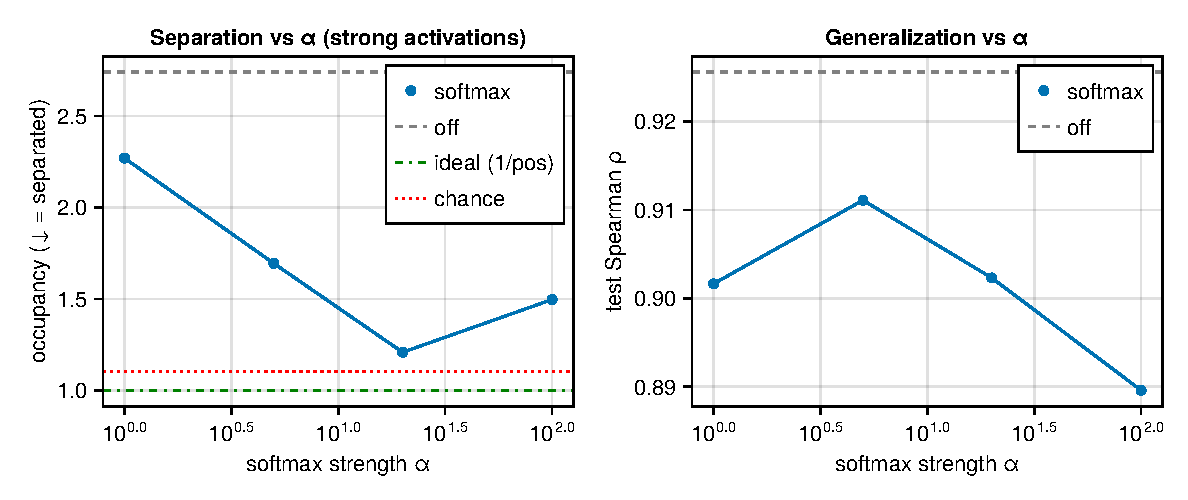
\includegraphics[width=0.95\textwidth]{figures/exp3_alpha.pdf}
\caption{Left: filter separation (occupancy, lower is more separated) vs.\ softmax strength
$\alpha$, with the operator-off and chance levels marked. Right: held-out accuracy (test
Spearman $\rho$) vs.\ $\alpha$. Together they show the separation/accuracy trade-off.}
\end{figure}

\section{Discussion}
\label{sec:disc}
\paragraph{Why it stops halfway.} The reason is baked into how the operator picks winners. It
runs a separate max \emph{per filter}: each filter looks at its own activations and keeps its
strongest spot in each window. Crucially, the filters never talk to each other. Nothing in the
math says ``filter B, that position is taken --- go somewhere else.'' So when a sequence
position is genuinely informative, every filter that responds to it keeps it, and they all pile
on. The operator thins out each filter's \emph{own} hits (within-filter non-overlap, which it
guarantees), but it never divides the territory \emph{between} filters.

\paragraph{Two levers that help --- and one that would finish the job.} Experiment~3 shows the
softmax strength $\alpha$ is a \emph{soft} version of exactly the fix we need. Raising $\alpha$
sharpens the over-channels softmax toward a per-position winner-take-all, and it does move
filters apart: occupancy falls from $2.8$ toward $2.4$ and exclusivity nearly triples. There is
a sweet spot around $\alpha=20$ where this separation is free of any held-out accuracy cost;
only at $\alpha=100$ does accuracy start to slip. A second, independent lever is simply
\emph{fewer filters}: dropping the inference layer from 20 to 10 filters (the bottleneck)
halved the crowding on its own. But neither closes the gap --- even $\alpha=100$ leaves
occupancy at twice chance. The \emph{hard} version would: a single winner per position across
all filters (a max \emph{across} channels instead of within each), a one-line change that forces
the territory to be split. Its risk is over-separation --- it may hurt tasks where nearby
filters \emph{should} co-fire, such as discovering motifs that genuinely co-occur at one site.

\paragraph{Annealing $\alpha$ is the natural next step.} The one place high $\alpha$ hurt was
training from scratch at $\alpha=100$. Ramping $\alpha$ up \emph{during} training --- let the
model first learn to fit at $\alpha=1$, then sharpen --- should reach high-$\alpha$ separation
without paying the accuracy tax. The knob is already in place (\texttt{sparse\_unpool\_alpha});
only a per-epoch schedule is missing.

\paragraph{The downstream cost is real.} At full length (Experiment~2), the sparsification
\emph{hurt} motif discovery: triplet groups collapsed from $11$ to $0$ and significant pairs
slipped from $8$ to $7$. This is the flip side of separation. The method finds co-occurring
motifs by looking for filters that fire together; the operator's whole job is to stop them
piling up, so it erases the joint firing the higher-order groups need. Separation and
co-occurrence discovery are, on this dataset, in direct tension --- which reframes the goal:
if the aim is co-occurrence, mild separation (small $\alpha$, or none) is safer than pushing it
hard.

\paragraph{Caveats.} Single dataset, single seed, an MSE regression proxy for training (not the
method's full objective), and one inference layer ($L^\star=1$, $p=5$). The occupancy gap
relative to chance is large and consistent across reruns, so the qualitative verdict is robust;
the exact numbers are not.


\end{document}
